% !TEX root =./main.tex

\section{Block 2: Calibration - Stentiford}

The calibration block detects the sonar transmissions, shifts the data in the time domain so that the start
 of the arrays line up with the transmit time, zeros out the transmission, and normalizes the received signal
 across the arrays. To determine where the transmission occurs, the block looks for 10 consecutive samples where
 the absolute value of the signal exceeds 0.08. Then, to determine where it ends, it waits for 30 consective
 samples with a level below 0.04. From there, it shifts the data left to align the array start with the
 transmission's start.
 
\begin{figure}[H]
    \centering
    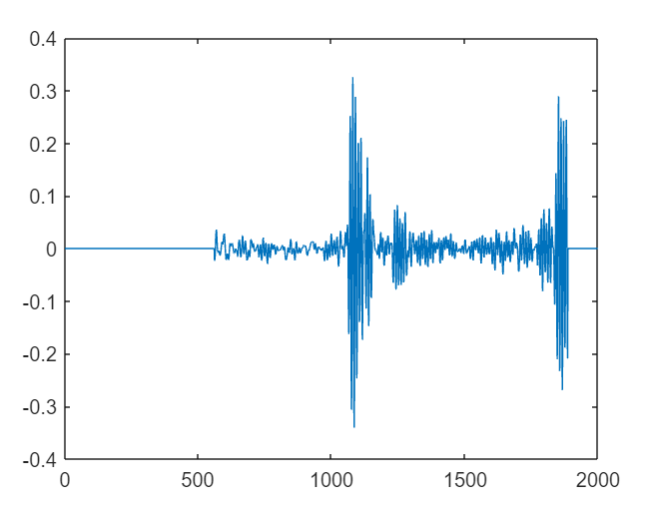
\includegraphics[width=0.5\linewidth]{figures/tx_zero.PNG}
    \caption{Transmission zeroed}
\end{figure}
 
 To normalize the signal magnitudes, the block examines four signals to find the maximum
 absolute values in each and applies the necessary gain to bring each signal up to the same strength as The
 strongest signal.

\begin{figure}[H]
    \centering
    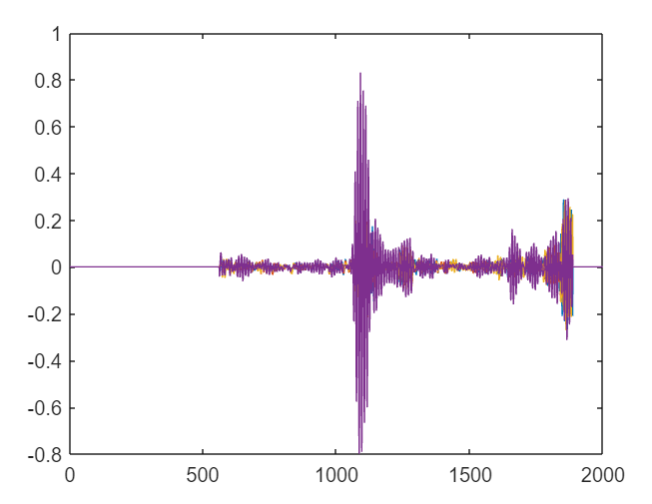
\includegraphics[width=0.5\linewidth]{figures/all_channels.PNG}
    \caption{All channels, pre-normalization}
\end{figure}

\begin{figure}[H]
    \centering
    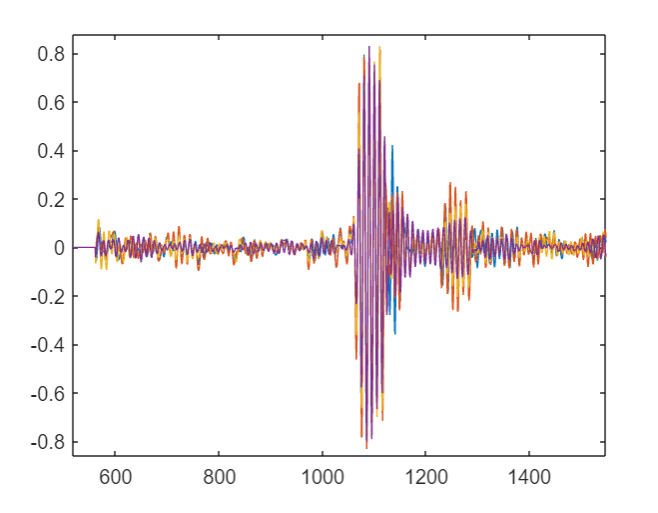
\includegraphics[width=0.5\linewidth]{figures/channels_normed.PNG}
    \caption{Channels normalized}
\end{figure}

To optimize for speed, the calibration stage was made into a unified module instead of a distinct stage 1a and
 stage 1b. By using the already-filtered signal, a much simpler (and therefore faster and less error-prone)
 approach was feasible. 

